\newpage
\section{Test of the Requirements of the Flanger and Chorus effects}

\subsection{Requirements \ref{req:flanger1} and \ref{req:chorus1}}

The requirement of having an \gls{lfo} that has a varying frequency between 0.1 and 10Hz has not been completely fulfilled. It has been tested that using 16-bits limits the \gls{cordic} algorithm to work with frequencies not less than \SI{1.7}{\hertz}. Switching to 32 bits to store \gls{cordic} data reduced this limit to 0.4 Hz which gives a working area for the \gls{lfo} frequency between 0.4 and 10Hz instead of 0.1 and 10Hz. This affects the chorus and the flanger together. In \autoref{app:cordic_shape} it proved that the \gls{cordic} algorithm is able to produce a \SI{0.4}{\hertz} sine wave.

\begin{figure}[hbt]
	\centering
  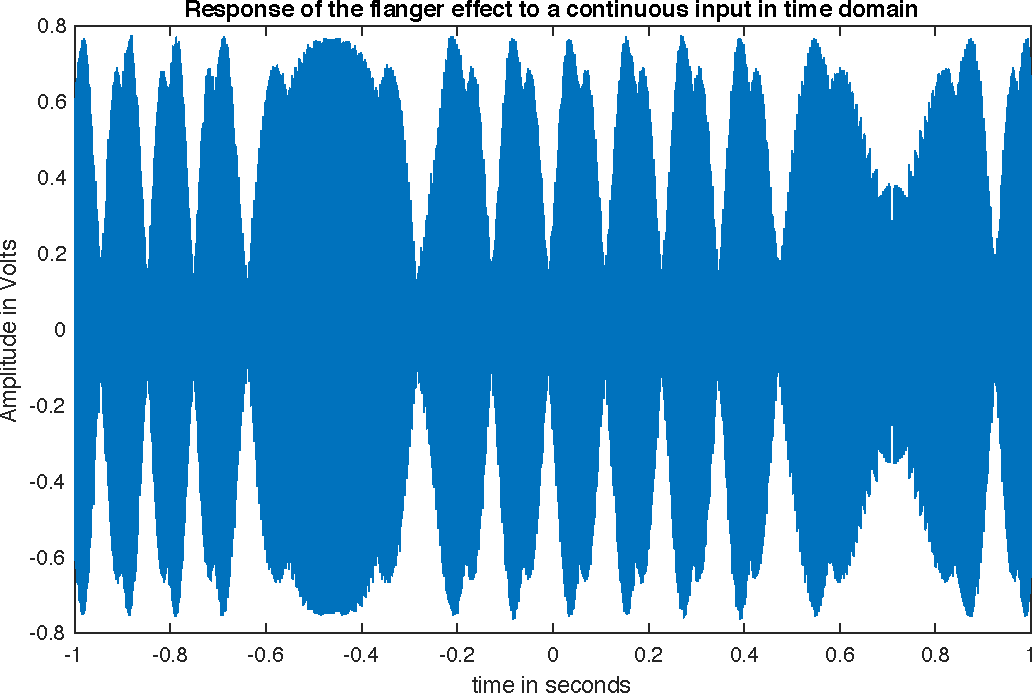
\includegraphics[width=1\textwidth]{flang_time_test.pdf}
  \caption{Time response of the implemented flanger effect}
  \label{fig:flang_time_test}
\end{figure}

It can be seen in figure \ref{fig:flang_time_test} that the \gls{lfo} is working since the delay is varying. This oval shape represents one \gls{lfo} sine period. In the attached Zip-file a video file called "flanger_impulse_response_test" shows the impulse response of the flanger effect.



\subsection{Requirement \ref{req:chorus2}}

According to \autoref{req:chorus2} the user must be able to choose the number of delay lines in the chorus effect. The chorus effect has been implemented in Assembly using macros, where each macro call represent a delay line. The user is free to choose how many times the macro should be called and thus choosing the number of delay lines. The user can also customize the gain and delay for each line which are the inputs of the macro. This is although only an option when changing it directly in the program since a user interface has not been implemented. Thus the requirement is partially approved.

\subsection{Requirement \ref{req:flanger2}}

According to \autoref{req:flanger2} the user must be able to change the gain of the flanger. This flexibility is made possible because the gain is called every time from the coefficient buffer, the value can then be changed there. The requirement is only partially approved since no user interface has been implemented. 





\begin{table}[H]
\centering
\caption{Recap of the requirements fulfilments for the chorus and flanger}
\label{test_of_flanger_table}
\begin{tabular}{|l|l|}
\hline
\rowcolor[HTML]{9B9B9B} 
\textbf{Requirement} & \textbf{Fulfilment State} \\ \hline
\textbf{\ref{req:flanger1}}    & \xmark                     \\ \hline
\textbf{\ref{req:chorus1}}    & \xmark                     \\ \hline
\textbf{\ref{req:chorus2}}    & \cmark*                     \\ \hline
\textbf{\ref{req:flanger2}}    & \cmark*                     \\ \hline
\end{tabular}
\end{table}
